\chapter{Caso de Estudio}
\section{Generador de Perfiles Energéticos}
El uso de los vehículos es particular al estilo de vida de cada usuario, tanto para vehículos de
combustión como para vehículos eléctricos. Por ello, es necesario generar perfiles energéticos que
sinteticen y agrupen los diferentes usos energéticos — y por tanto la necesidad de carga de dichos
vehículos — de los usuarios.\\

En el primer bloque que compone el trabajo, se ha desarrollado un algoritmo generador de perfiles 
de carga de EVs, partiendo del \textit{Electric Vehicle Charging Dataset}~\cite{kaggle_ev_charging_patterns}.
A partir de este dataset, se han generado nuevas muestras sintéticas de perfiles de carga y uso 
típico de las estaciones de carga. Para ello, se ha utilizado una de las herramientas de IA 
Generativa, presentada en el Capítulo~\ref{chapter:chapter2}, concretamente se ha hecho uso de una
GAN.\\

Los parámetros de la GAN se han ajustado para que los perfiles generados representen adecuadamente
la variabilidad de la demanda energética para la carga de un EV, teniendo en cuenta las restricciones,
requisitos y hábitos del usuario. El resultado es un conjunto de perfiles energéticos que pueden
ser utilizados para entrenar y evaluar el gestor de carga de EVs, así como para simular diferentes
escenarios de carga y consumo energético.\\

A partir de los datos obtenidos, tanto del dataset original como los generados, se han podido 
extraer una serie de perfiles y patrones de consumo energético, que se han agrupado en distintas 
categorías, y que se han utilizado para entrenar el gestor de carga de EVs. Estos perfiles se han
usado principalmente para ofrecer al gestor un rango de disponibilidad de carga del vehículo y 
oportunidades de carga a lo largo del día, en funcion de la "personalidad" de cada uno de los 
usuarios.\\

Es importante resaltar que, con el fin de introducir algo de variabilidad en los perfiles, y reducir
el determinismo en cuanto a la disponibilidad de carga se refiere, durante el proyecto se ha 
tratado esta funcion de disponibilidad como una función probabilística definida a trozos. Esto 
significa que, para cada perfil de usuario, según la hora del día, se ha asignado una probabilidad
de que el usuario esté disponible para cargar su vehículo eléctrico. El número concreto de esta
probabilidad asignada, se ha obtenido juntando la la información del dataset original, la 
información obtenida de los datos generados, y la idea general detrás de cada perfil de usuario, y
sus características más convencionales.\\

Los perfiles generados se han agrupado en las siguientes categorías, que representan los
distintos tipos de usuarios y sus hábitos de carga:
\begin{table}[H]
    \centering
    \begin{tabular}{p{2cm} p{7cm} p{3.5cm}}
        \toprule
        \textbf{Perfil} & \textbf{Hábitos de carga} & \textbf{Disponibilidad (probabilidad)} \\
        \midrule
        Trabajador (\texttt{worker}) &
        Carga principalmente de noche (00:00–06:00, 21:00–00:00); baja disponibilidad en horario laboral. &
        00:00–06:00: 0.95; 06:00–21:00: 0.10; 21:00–00:00: 0.85 \\
        \addlinespace[0.5ex]
        Flexible &
        Disponibilidad media y estable, con ligera bajada en horario laboral. &
        00:00–08:00: 0.80; 08:00–18:00: 0.60; 18:00–00:00: 0.75 \\
        \addlinespace[0.5ex]
        Jubilado (\texttt{retired}) &
        Alta disponibilidad todo el día, salvo ausencias puntuales a mediodía y tarde. &
        00:00–12:00: 0.95; 12:00–16:00: 0.70; 16:00–00:00: 0.90 \\
        \addlinespace[0.5ex]
        Viajero (\texttt{traveller}) &
        Alta disponibilidad salvo ausencias frecuentes en horario diurno y algunas tardes. &
        00:00–08:00: 0.90; 08:00–18:00: 0.40; 18:00–00:00: 0.80 \\
        \addlinespace[0.5ex]
        Nocturno (\texttt{night\_owl}) &
        Carga casi exclusiva por la noche; baja disponibilidad diurna. &
        00:00–06:00: 0.98; 06:00–20:00: 0.15; 20:00–00:00: 0.90 \\
        \bottomrule
    \end{tabular}
    \caption{Perfiles energéticos generados para usuarios de EV y sus probabilidades de disponibilidad}
\end{table}

\section{Generador de Consumo}
Este segundo bloque se centra en la tarea de generación de consumos energéticos domésticos,
utilizando el software \textit{Load Profile Generator (LPG)}. Se ha configurado una vivienda de
tipo unifamiliar en el entorno urbano de Madrid, modelada para representar una situación típica
de un hogar con presencia de vehículo eléctrico, hijos y hábitos laborales estándar. La configuración
empleada es la siguiente:

\begin{table}[H]
    \centering
    \begin{tabular}{p{4cm} p{9.8cm}}
        \\[-1.5ex] % Espacio extra antes de la primera fila
        \toprule
        \textbf{Parámetro} & \textbf{Descripción} \\
        \midrule
        Tiempo simulado & 365 días (1 año completo) \\
        \\[-1.5ex]
        Resolución temporal interna & 1 minuto \\
        \\[-1.5ex]
        Resolución temporal externa & 15 minutos \\
        \\[-1.5ex]
        Ubicación geográfica & Madrid, España \\
        \\[-1.5ex]
        Tipo de vivienda & Unifamiliar, tamaño medio (100–150 m\textsuperscript{2}), con garaje y trastero \\
        \\[-1.5ex]
        Aislamiento térmico & Estándar \\
        \\[-1.5ex]
        Equipamiento & Completo en electrodomésticos \\
        \\[-1.5ex]
        Composición familiar &
        \begin{itemize}[noitemsep, topsep=-10pt]
            \item Mujer (trabaja fuera, jornada completa)
            \item Hombre (trabaja en casa, jornada parcial)
            \item Niños: uno en edad escolar, otro en edad preescolar
        \end{itemize} \\
        \\[-1.5ex]
        Vehículo eléctrico &
        \begin{itemize}[noitemsep, topsep=-10pt]
            \item Un coche compartido
            \item Uso diario laboral y escolar
            \item Carga preferente nocturna
        \end{itemize} \\
        \\[-1.5ex]
        Perfil de temperatura & Datos realistas para 2025 en Madrid \\
        \\[-1.5ex]
        Calendario & Incluye fines de semana y festivos nacionales \\
        \bottomrule
    \end{tabular}
    \caption{Parámetros de configuración de la vivienda en LPG}
\end{table}
La vivienda, como se muestra en la anterior tabla, está ocupada por cuatro personas, cuyas rutinas 
diarias han sido configuradas para representar un hogar realista con uso intensivo de energía:

\begin{itemize}
    \item \textbf{Adulto 1 (mujer):} trabaja fuera del hogar a jornada completa (8h–17h),
    desplazándose en vehículo eléctrico cinco días a la semana. Contribuye a la carga del
    EV en horario nocturno.

    \item \textbf{Adulto 2 (hombre):} trabaja parcialmente desde casa, con jornada reducida.
    Su presencia en el hogar durante el día impacta en el uso de climatización, cocina y
    dispositivos electrónicos.

    \item \textbf{Niño 1:} escolarizado, con jornada matinal completa. Genera picos de consumo
    por la mañana y por la tarde (actividades, ducha, iluminación).

    \item \textbf{Niño 2:} edad preescolar, cuidado en casa. Su presencia constante condiciona
    el uso continuo de climatización, iluminación y aparatos electrónicos de ocio.
\end{itemize}
Con estas características cargadas en la configuración del programa generador, se ha procedido a la
generación de los siguientes datos de consumo energético:

\begin{table}[H]
\centering
    \begin{tabular}{@{}p{3.4cm} p{10.6cm}@{}}
        \toprule
        \textbf{Categoría} & \textbf{Descripción} \\
        \midrule
        Electrodomésticos de cocina &
        Horno, vitrocerámica, microondas; lavavajillas; frigorífico y congelador (consumo continuo) \\
        \\[-1.5ex]
        Electrodomésticos de limpieza & Lavadora, secadora y aspiradora \\
        \\[-1.5ex]
        Entretenimiento y oficina &
        Televisores, ordenadores, router; consolas, altavoces, impresoras \\
        \\[-1.5ex]
        Iluminación &
        Luz general por estancias, activación dependiente de presencia y hora del día \\
        \\[-1.5ex]
        Climatización &
        Calefacción eléctrica (invierno); aire acondicionado o ventiladores (verano) \\
        \\[-1.5ex]
        Agua caliente sanitaria (ACS) &
        Consumo eléctrico en ausencia de caldera de gas \\
        \\[-1.5ex]
        Carga del vehículo eléctrico &
        Carga según trayectos diarios; horarios preferentes nocturnos \\
        \\[-1.5ex]
        Consumo en espera (stand-by) &
        Dispositivos conectados permanentemente; carga latente (TV, router, cargadores)\\
        \bottomrule
    \end{tabular}
\caption{Categorías de consumo energético simuladas}
\end{table}
Con esta configuración se han generado los consumos energéticos horarios agregados para los 
distintos elementos. Este perfil de consumo no gestionable sirve como input para el gestor 
inteligente de carga, presentado en la siguiente sección.

\subsubsection{Descripción de los Datos Generados}
A continuación se muestran algunas de las gráficas generadas por la aplicación, que describen los datos generados
por el LPG. Estas gráficas muestran el consumo energético de la vivienda a lo largo de un año,
con una resolución de 15 minutos.
\begin{figure}[H]
    \centering
    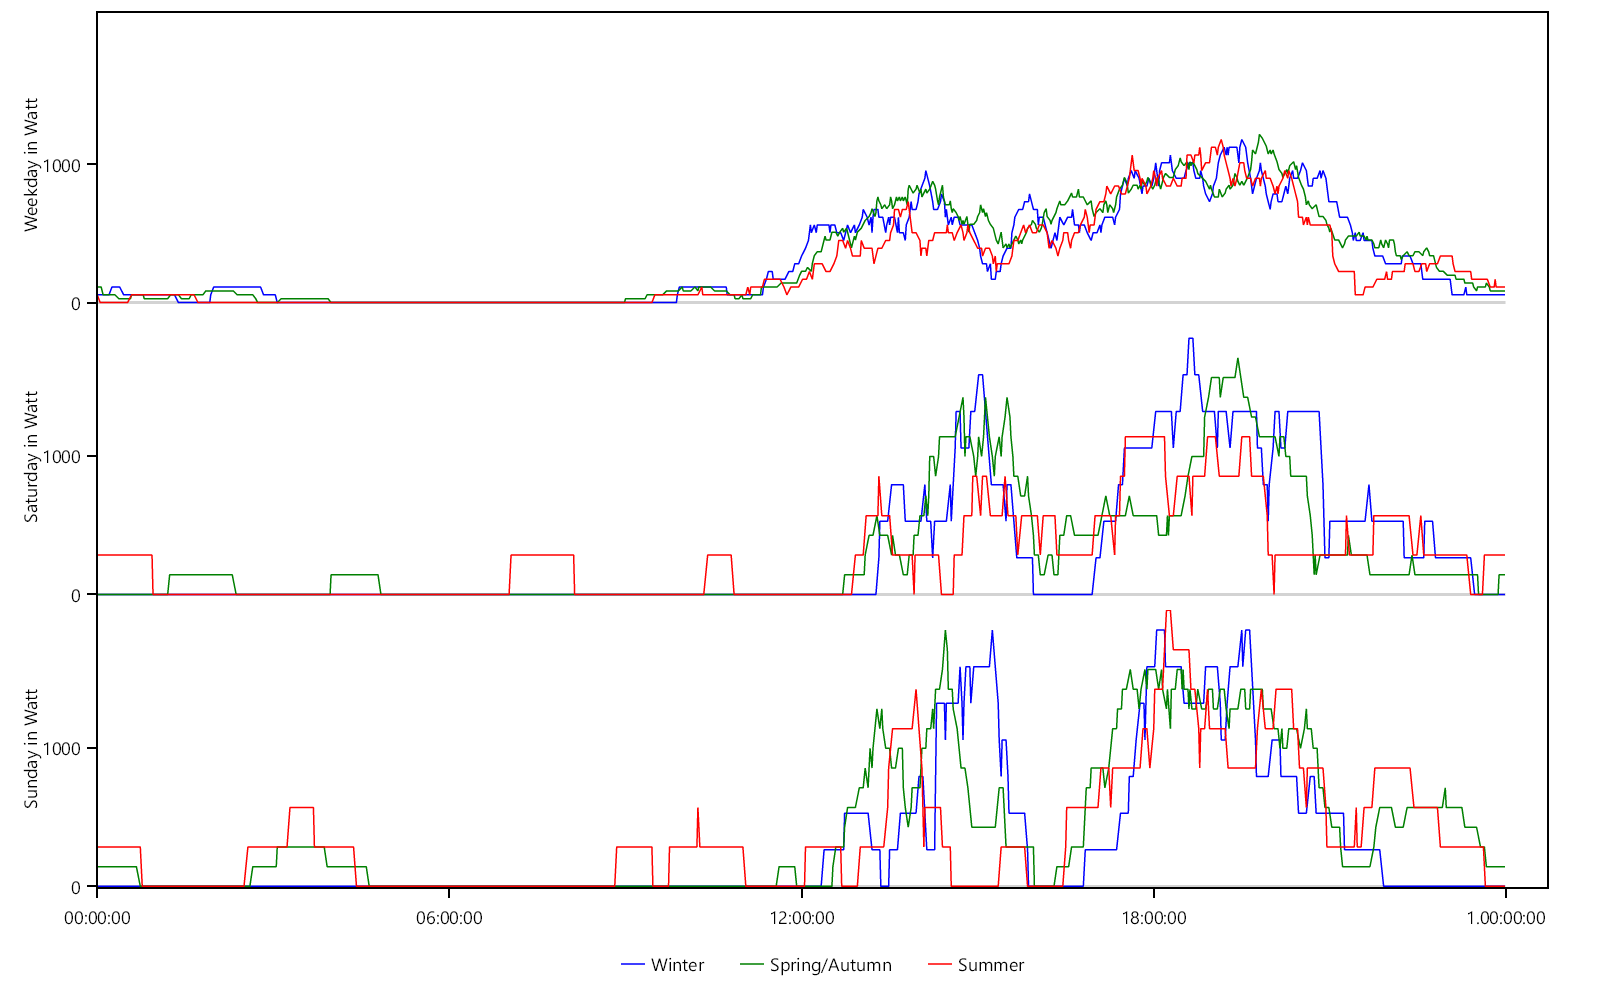
\includegraphics[width=0.4957\textwidth]{images/LPG/WeekdayProfiles.Electricity for Car Charging.png}
    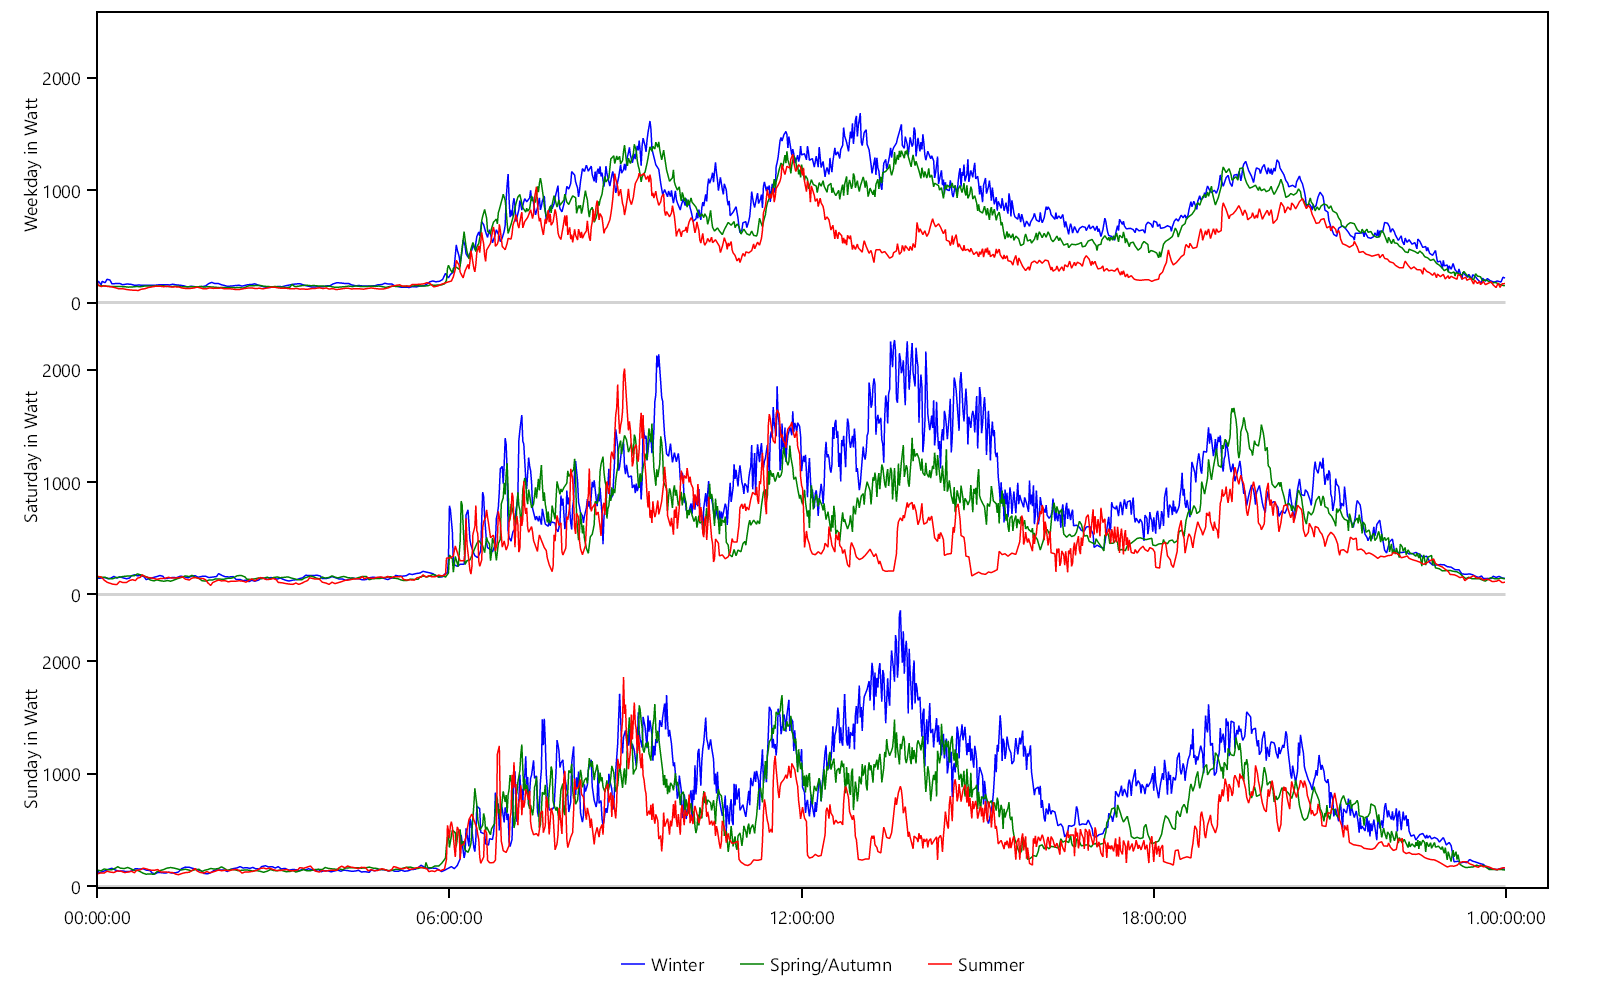
\includegraphics[width=0.4957\textwidth]{images/LPG/WeekdayProfiles.Electricity.png}
    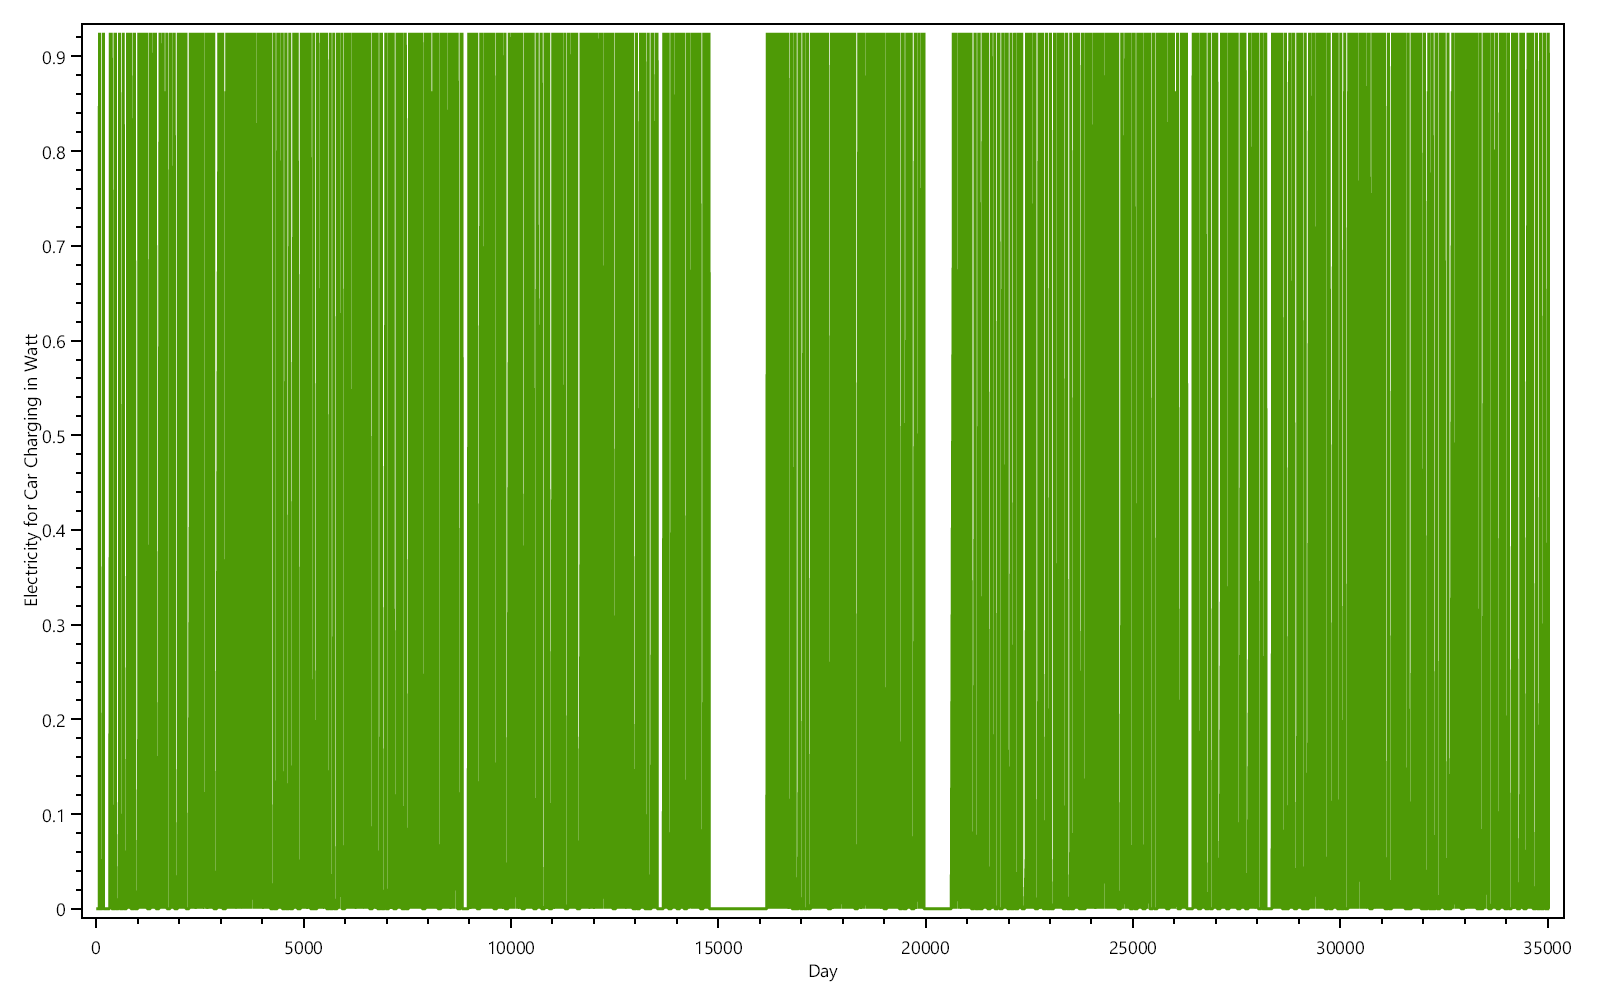
\includegraphics[width=0.4957\textwidth]{images/LPG/SumProfiles_900s.Electricity for Car Charging.png}
    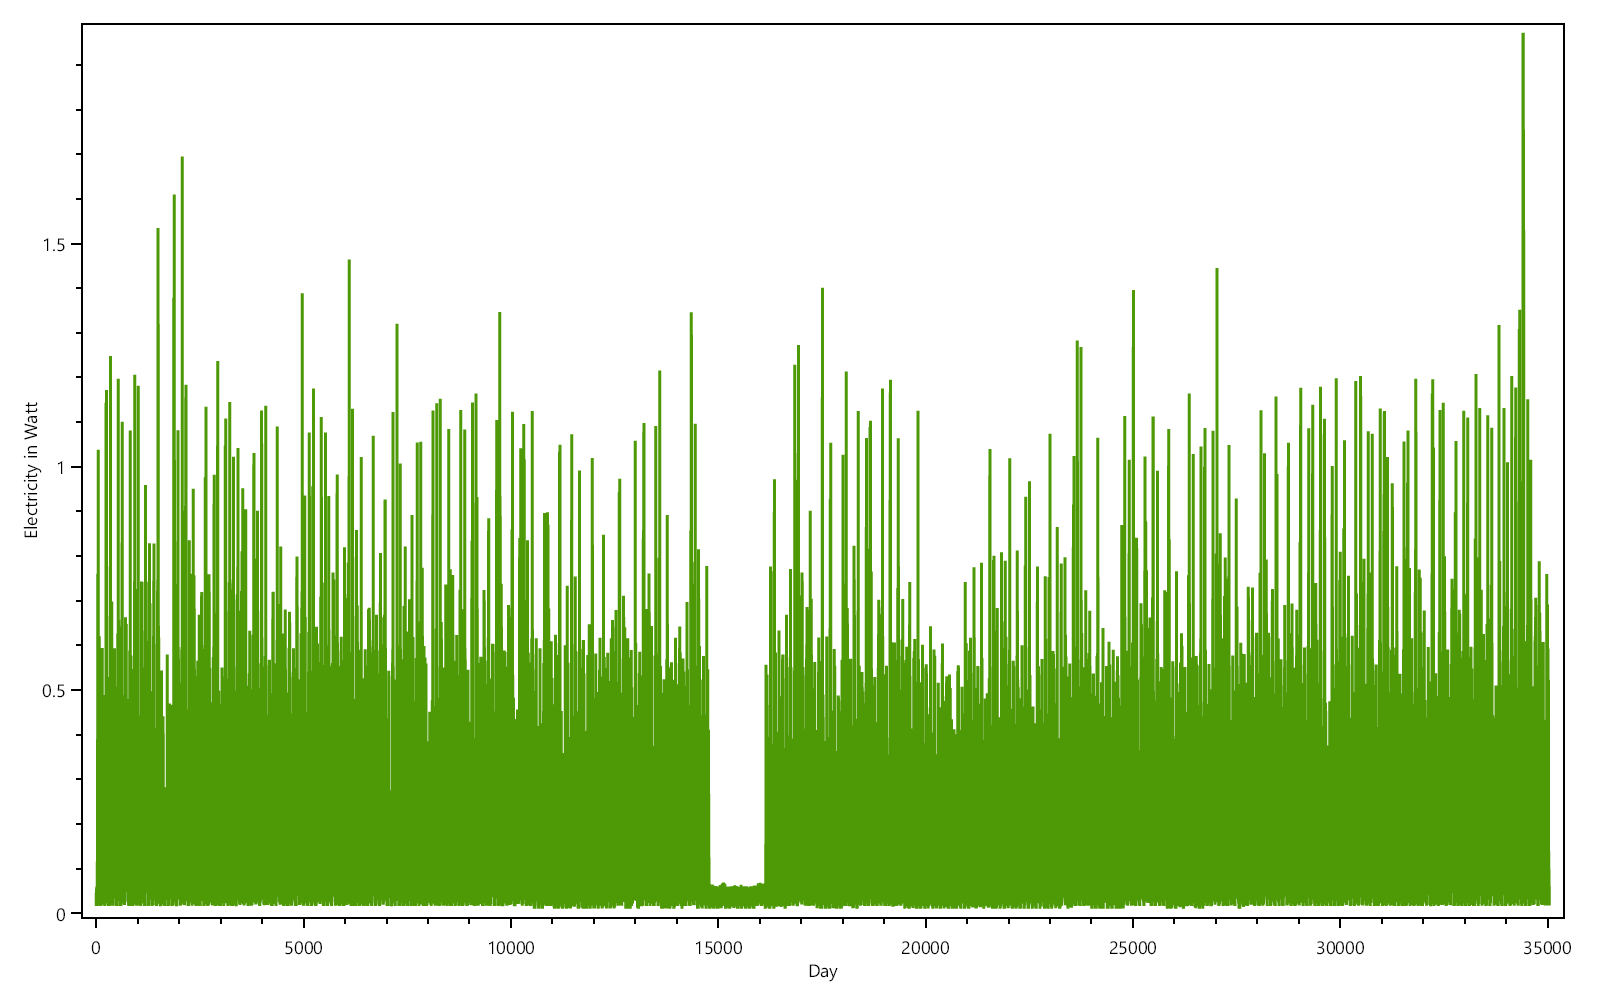
\includegraphics[width=0.4957\textwidth]{images/LPG/SumProfiles_900s.Electricity.png}
    \caption{Gráficas generadas por el LPG.}
    \label{fig:lpg_consumo}
\end{figure}

Las dos primeras gráficas muestran el consumo energético de la vivienda, promediado a lo largo de 
un año, durante los días laborables de la semana y el fin de semana. La gráfica de la izquierda 
muestra el consumo energético para la carga del vehículo eléctrico, mientras que la gráfica de la 
derecha muestra el consumo total de energía de la vivienda. Además, se han representado las 
distintas estaciones del año con líneas de distinto color, para un análisis más detallado.\\

Las gráficas en la fila inferior muestran el consumo total de energía para la carga del EV, y en
general a lo largo del año, respectivamente. Se puede observar que el consumo energético varía a lo 
largo del año, con picos de consumo en invierno y verano, y una tendencia general de aumento del 
consumo a lo largo del año.\\

Estas gráficas, siendo una muestra de todas las disponibles para el análisis, proporcionan una 
visión general del consumo energético de la vivienda, y son útiles para entender los patrones de
consumo y carga del vehículo eléctrico. Además, permiten identificar los momentos de mayor
consumo energético, lo que es esencial para la gestión eficiente de la carga del EV.\\

Más imágenes de las gráficas generadas por el LPG, y análisis propios, se pueden encontrar en el
anexo~\ref{annex:annex1}.

\section{Gestor de Carga de EVs}
El gestor de carga es el tercer y último bloque del trabajo, y es realmente el foco del mismo. 
Para su desarrollo, se ha implementado una red neuronal de aprendizaje por refuerzo DQN, que se ha 
entrenado con los perfiles de consumo energético, obtenidos tras la generación de datos adicionales, 
y toda la información de la vivienda y del vehículo eléctrico.\\

El gestor de carga tiene como objetivo optimizar la carga del vehículo eléctrico, minimizando por 
supuesto el coste incurrido en la carga, teniendo en cuenta las restricciones y requisitos del usuario. 
Para ello, se ha implementado un algoritmo de aprendizaje por refuerzo, que permite al gestor de carga 
aprender de la experiencia y mejorar su rendimiento a lo largo del tiempo.\\

Antes de usar redes neuronales, se ha implementado un algoritmo de optimización clásico, que
sirve como base para comparar el rendimiento del gestor de carga. Este algoritmo utiliza las 
técnicas de optimización clásica, tal y como se ha presentado en el Capítulo~\ref{chapter:chapter2}, 
para obtener una solución óptima al problema que presenta la carga del EV.\\

\subsection{Optimización Clásica}
Primeramente, se han de definir el conjunto de variables que después formarán las restricciones y
objetivos del problema de optimización. En este caso, las variables son las siguientes:
\begin{itemize}
    \item $\mathit{P}(t)$: Potencia en el instante $t$ [kW]
    \item $\mathit{E}(t)$: Energía en el instante $t$ [kWh]
    \item $P_\text{Max}$: Potencia máxima en el cargador [kW]
    \item $\mathit{SOC}(t)$: Estado de carga en el instante $t$ [kWh]
    \item $P_{NG}(t)$: Potencia del No Gestionable en $t$ [kW]
    \item $\eta$: Eficiencia del sistema
    \item $A(t)$: Disponibilidad en el instante $t$ [1: disponible, 0: no]
    \item $p(t)$: Precio de la electricidad en el instante $t$ [€/kWh]
    \item $C(t)$: Coste de carga en el instante $t$ [€]
\end{itemize}

Una vez se tienen claras las variables, tras un análisis del problema, se definen las siguientes
restricciones y función objetivo:
\begin{align}
    \min_{P(t)} \quad & \sum_{t} C(t) = \sum_{t} E(t) \cdot p(t) \label{eq:objective_cost} \\[6pt]
    \text{s.a.} \quad & 0 \leq P(t) \leq P_{\text{max}} \cdot A(t) \label{eq:charging_window} \\[6pt]
    & P(t) + P_{\text{NG}}(t) \leq P_{\text{red}} \label{eq:grid_limit} \\[6pt]
    & SOC(t+1) = SOC(t) + \eta \cdot \frac{P(t) \cdot \Delta t}{\text{capacidad}} \label{eq:soc_update} \\[6pt]
    & \sum_{t} P(t) \cdot \Delta t \geq (SOC_f - SOC_i) \cdot \text{capacidad} \label{eq:soc_requirement}
\end{align}
 
Una vez ya se ha planteado el problema, se implementa el Python~\cite{python2024language}
usando la librería \textit{Pyomo}~\cite{pyomo2024} para definir el modelo de optimización, y
\textit{GurobiPy}~\cite{gurobi2024} como solver. El código se ha implementado de forma que se pueda
cargar el perfil de consumo energético generado por el LPG, y se pueda ejecutar el algoritmo de
optimización para obtener la solución óptima al problema de carga del EV.\\

Los resultados obtenidos con este algoritmo de optimización clásico sirven como base para
comparar el rendimiento del gestor de carga basado en aprendizaje por refuerzo, y para evaluar la
mejora en la eficiencia y reducción de costes que se puede lograr con el uso de técnicas del RL.\\ 

Los resultados obtenidos con el algoritmo de optimización clásico se muestran a continuación:

%%% INSERTAR RESULTADOS OBTENIDOS CON EL ALGORITMO DE OPTIMIZACIÓN CLÁSICO %%%

\subsection{Red Neuronal de Aprendizaje por Refuerzo}
Para la implementación del gestor, se ha usado una red neuronal de aprendizaje por refuerzo DQN-LSTM, 
entrenada con los mismos datos que el algoritmo de optimización clásico, es decir, los perfiles de
consumo energético generados por el LPG, y la información de la vivienda y del vehículo eléctrico. 
En cierta forma, tal y como se ha explicado en el Capítulo~\ref{chapter:chapter2}, las redes 
neuronales pueden ser concebidas, en esencia, como un sistema aproximador de funciones. Por lo 
tanto, el diseño de la red neuronal irá muy en línea con la estructura del problema de optimización
clásico, y las variables que se han definido anteriormente.\\

El modelo propuesto se estructura en varias capas secuenciales, diseñadas para procesar información
temporal y generar una salida final. La arquitectura se compone de los siguientes bloques:
\begin{itemize}
    \item \textbf{Capa LSTM}: Una capa tipo LSTM (\texttt{nn.LSTM}) que permite procesar secuencias 
    de datos temporales, aprendiendo relaciones a lo largo del tiempo. Toma como entrada el tamaño 
    de los vectores (\texttt{input\_dim}), el tamaño del estado oculto (\texttt{hidden\_dim}) y el 
    número de capas apiladas (\texttt{lstm\_layers}, por defecto serán 2).
    
    \item \textbf{Normalización de capa}: Después de la LSTM, se aplica una normalización 
    (\texttt{nn.LayerNorm}) para estabilizar el entrenamiento y mejorar la convergencia del modelo.

    \item \textbf{Primera capa totalmente conectada}: Una capa lineal (\texttt{nn.Linear}) transforma 
    la salida de la LSTM, manteniendo la dimensión oculta. Actúa como parte del bloque de decisión 
    del modelo.

    \item \textbf{Dropout}: Se introduce una capa de regularización (\texttt{nn.Dropout}) con 
    probabilidad 0.2 para evitar sobreajuste, desactivando aleatoriamente algunas neuronas durante 
    el entrenamiento.

    \item \textbf{Segunda capa totalmente conectada}: Otra capa lineal que sigue procesando la 
    representación interna, manteniendo la dimensión.

    \item \textbf{Segunda normalización}: Se aplica una nueva normalización de capa para estabilizar 
    las activaciones antes de la salida final.

    \item \textbf{Capa de salida}: Finalmente, una capa lineal proyecta la representación latente 
    al tamaño deseado de la salida (\texttt{output\_dim}), adaptada al problema.
\end{itemize}

\begin{figure}[H]
    \centering
    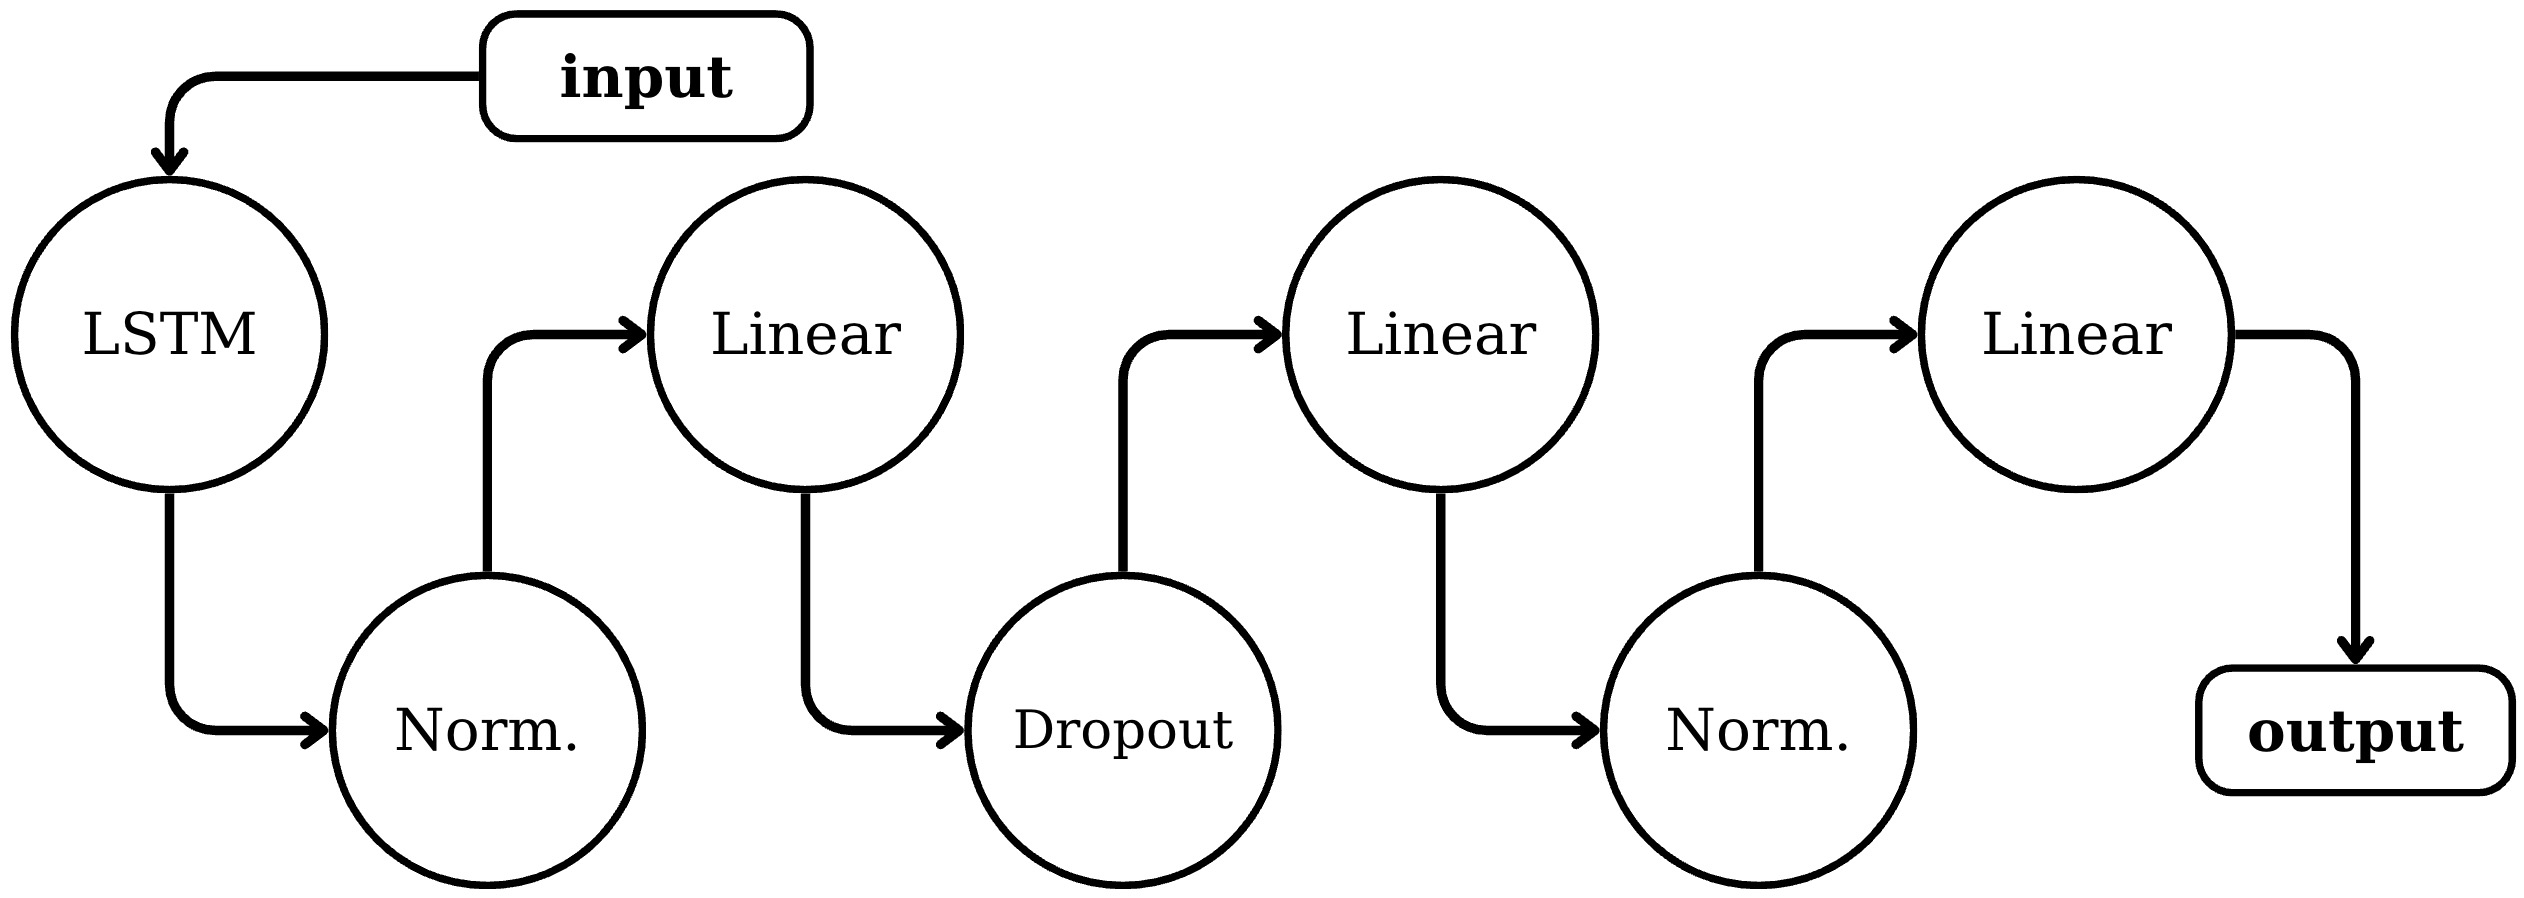
\includegraphics[width=1\textwidth]{images/gestor_arch.png}
    \caption{Arquitectura de la red neuronal DQN utilizada en el gestor de carga. Fuente: 
    Elaboración propia.}
    \label{fig:arch_dqn}
\end{figure}

\subsubsection{Entorno de la Red DQN-LSTM}
Para entrenar y evaluar el comportamiento del agente gestor, se ha desarrollado un entorno 
personalizado en Python~\cite{python2024language}. Este entorno representa un hogar con un vehículo 
eléctrico, y tiene en cuenta tanto el consumo energético no gestionable como la disponibilidad  del 
EV y el precio de la electricidad en cada intervalo de tiempo.

\paragraph{Estado del entorno.}
El vector de estado \(\mathbf{s}_t \in \mathbb{R}^5\) en cada instante \(t\) incluye las siguientes 
variables:
\begin{itemize}
    \item \textbf{State of Charge (SOC):} estado de carga actual del vehículo eléctrico.
    \item \textbf{Hora normalizada:} instante del día en formato continuo \([0, 1]\).
    \item \textbf{Consumo no gestionable (\(P_{NG}\)):} potencia usada por la vivienda que no se 
    puede desplazar.
    \item \textbf{Disponibilidad (\(A_t\)):} probabilidad de que el vehículo esté conectado en ese 
    instante.
    \item \textbf{Precio de la electricidad:} coste por kWh en el instante actual.
\end{itemize}

\paragraph{Acciones.} 
La acción es binaria \(a_t \in \{0, 1\}\), indicando si se decide cargar (1) o no cargar (0) 
durante el intervalo actual de 15 minutos.

\paragraph{Dinámica.} 
Dado un estado y una acción, se debe calcular el nuevo estado del entorno, que desencadena dicha 
accion. Esto significa que el entorno debe calcular:
\begin{itemize}
    \item La potencia solicitada \(P = a_t \cdot P_{\text{max}}\).
    \item La energía cargada, ajustada a las restricciones físicas y de disponibilidad.
    \item La actualización del SOC: 
    \(\Delta SOC = P \cdot \Delta t\), con \(\Delta t = 0{,}25~\text{h}\).
    \item El coste de la carga en ese instante: \(C_t = P \cdot p(t)\).
    \item La recompensa obtenida, que depende de la acción tomada y del estado del entorno.
\end{itemize}

\paragraph{Función de recompensa.} 
La recompensa está diseñada para reflejar los objetivos del sistema: minimizar el coste energético, 
evitar violaciones de restricciones físicas, y alcanzar el SOC deseado al final del día. Se 
penaliza explícitamente el uso de energía cuando el vehículo no está disponible o cuando se supera 
el margen permitido por la potencia contratada. Por tanto, se penalizará al agente en los siguientes
casos:
\begin{itemize}
    \item Coste de la electricidad en ese instante.
    \item Cargar cuando el vehículo no está disponible (\(A_t \approx 0\)).
    \item Superar la potencia contratada (\(P > P_{\text{red}} - P_{NG}\)).
    \item Exceder el SOC máximo deseado, si la batería ya se ha cargado a ese nivel.
\end{itemize}

Adicionalmente, se recompensa positivamente al agente si el SOC final se encuentra en el rango 
deseado (\([0{,}75;0{,}8]\), por ejemplo) al término del episodio. Pr tanto, la función de 
recompensa \(R_t\) se puede expresar maremáticamente como:
\begin{equation}
    r_t = -\left( C_t + \lambda_1 \cdot A_t + \lambda_2 \cdot (P - P_{\text{red}} + P_{NG})^2 +
    \lambda_3 \cdot (SOC - SOC_{\text{max}})^2 \right)
\end{equation}

donde \(\lambda_1\), \(\lambda_2\) y \(\lambda_3\) son coeficientes de ponderación que ajustan la
importancia de cada componente de la recompensa. El coste \(C_t\) se calcula como el producto 
de la potencia entregada \(P\) y el precio de la electricidad \(p(t)\) en el instante \(t\).

\paragraph{Formato del episodio.}  
Cada episodio simula un día completo dividido en intervalos de 15 minutos (96 pasos). El SOC se 
inicializa aleatoriamente entre 3\% y 25\% al inicio del día, y se va actualizando conforme a las 
decisiones del agente.

\subsubsection{Entrenamiento del Agente DQN-LSTM.}  
Durante el entrenamiento, el agente observa secuencias de estados \((s_{t-T}, \ldots, s_t)\) para 
estimar la utilidad esperada de ejecutar cada acción \(a \in \{0, 1\}\). La red neuronal devuelve 
dos valores, que serían la acción de cargar o no cargar el vehículo en el intervalo actual.

\paragraph{Representación temporal.}  
Para aportar contexto al momento de la carga, la disponibilidad y precio, de manera que no sea un 
análisis puntual de la situación, se utiliza una secuencia de entrada temporal de longitud 
\(T = 4\) pasos (1 hora), alimentada a través de la capa LSTM.

\paragraph{Parámetros del entrenamiento.}  
El entrenamiento se realiza durante \(N = 365\) episodios completos (días), con los siguientes 
hiperparámetros base:
\begin{itemize}
    \item \textbf{Tasa de aprendizaje (\(\alpha\))}: 0.001
    \item \textbf{Factor de descuento (\(\gamma\))}: 0.95
    \item \textbf{Exploración inicial (\(\epsilon\))}: 0.1, decreciendo progresivamente
    \item \textbf{Tamaño del batch}: 64
    \item \textbf{Tamaño de la secuencia temporal}: 4 pasos
    \item \textbf{Tamaño del buffer de experiencia}: 10000
\end{itemize}

Para la elección de los valores de estos hiperparámetros, se ha realizado una algoritmo de 
\textit{Grid Search} sobre un rango de valores, y se ha seleccionado el conjunto que mejor 
rendimiento ha obtenido en términos de recompensa media acumulada y estabilidad del aprendizaje.

\paragraph{Algoritmo.}  
Se emplea el algoritmo clásico de \textit{Deep Q-Learning} con \textit{replay buffer}, que incluye
actualizaciones periódicas de la red objetivo, y política \(\epsilon\)-greedy. El error se calcula 
mediante pérdida MSE (\textit{Mean Squared Error}, Error Cuadrático Medio) entre la estimación del 
valor actual y el objetivo de Bellman, tal y como se ha presentado en el Capítulo~\ref{chapter:chapter2}.

\paragraph{Monitorización y métricas.}  
Durante el entrenamiento, se muestra una barra de progreso en terminal, y se registran métricas 
como recompensa promedio por episodio. También se exportan ficheros \texttt{.csv} de depuración con 
los valores de potencia aplicada, SOC, precio y recompensas en cada paso, permitiendo inspeccionar 
el comportamiento del agente en detalle.

\subsubsection{Resultados del Agente DQN-LSTM.}
Los resultados obtenidos por el agente gestor, después del entrenamiento, se muestran a continuación.
